\documentclass[../main.tex]{subfiles}

\begin{document}

\chapter[Resilient Primal Decomposition-based dMPC for scarce systems]{Resilient \\Primal Decomposition-based \\distributed \\Model Predictive Control\\ for scarce systems}\label{sec:safe_pddmpc_eq}
\epigraph{\centering So you tell me 'trust me' \\I can trust you\\ Just let me show you \\But I gotta work it out in a shadow of doubt \\'Cause I don't know if I know you}
{\textit{Lie}\\\textsc{Kevin Moore}}

In this chapter, we focus on the analysis of the primal decomposition-based \dmpc{} problem for scarce systems when in the presence of the attack chosen in~\S\ref{sec:anomalous}.

With the knowledge acquired after the analysis, we propose a method to detect the attacks and mitigate its effects.

\minitoc


\section{Scarce systems under attack}\label{sec:analys-scarce-syst}

Different from~\cite{VelardeEtAl2018,MaestreEtAl2021} which propose robust solutions, we propose a resilient \dmpc{} based on a hybrid of analytical/learning active detection method.
For this end, we begin with an analysis of the system under attack.

\subsection{Scarce Systems}\label{sec:scarce-systems}
First we recall the monolithic \mpc{} equivalent problem~\eqref{eq:qp_standard_form}, once more reproduced for the reader's convenience,
\begin{equation}
  \label{eq:qp_standard_form_again}
  \tag{\ref*{eq:qp_standard_form}}
  \begin{aligned}
    \begin{matrix}
      \minimize\limits_{\vec{U}[k]} &
                                                 \frac{1}{2}\norm{\vec{U}[k]}^{2}_{H} + {\vec{f}[k]}^{T}\vec{U}[k] &\\
      \mathrm{subject~ to} &
                             \bar{\Gamma}\vec{U}[k]\preceq {\vec{U}}_{\text{max}}
    \end{matrix}
  \end{aligned},
\end{equation}
and the local problems~\eqref{eq:DOP_local} solved in the primal decomposition, also reproduced,

\begin{equation}
  \label{eq:DOP_local_reprise}
  \tag{\ref*{eq:DOP_local}}
  \bar{J}_{i}^{\star}(\thetaik)=
  \begin{matrix}
    \minimize\limits_{\vec{U}_{i}[k]}&\obji=\frac{1}{2}\norm{\vec{U}_{i}[k]}^{2}_{H_{i}} + {\vec{f}_{i}[k]}^{T}\vec{U}_{i}[k]\\
    \mathrm{subject~ to} & \bar{\Gamma}_{i}\vec{U}_{i}[k] \preceq \thetaik:\lambdaik
  \end{matrix}.
\end{equation}

The unconstrained version of problems~\eqref{eq:qp_standard_form_again} and~\eqref{eq:DOP_local_reprise} are
\begin{align}
  \label{eq:qp_standard_form_unconstrained}
  \begin{aligned}
    \begin{matrix}
      \minimize\limits_{\vec{U}[k]} &
                                                 \frac{1}{2}\norm{\vec{U}[k]}^{2}_{H} + {\vec{f}[k]}^{T}\vec{U}[k] &\\
    \end{matrix},
  \end{aligned}\\
  \label{eq:DOP_local_unconstrained}
  \begin{aligned}
    \begin{matrix}
    \minimize\limits_{\vec{U}_{i}[k]}&\frac{1}{2}\norm{\vec{U}_{i}[k]}^{2}_{H_{i}} + {\vec{f}_{i}[k]}^{T}\vec{U}_{i}[k]\\
    \end{matrix},
  \end{aligned}
\end{align}
and have analytical solutions~\cite{BoydVandenberghe2004}
\begin{align}
  \label{eq:qp_standard_form_unconstrained_solution}
  \vec{U}_{\text{unc}}^{\star}[k]=-H^{-1}\vec{f}[k],\\
  \label{eq:DOP_local_unconstrained_solution}
  \vec{U}_{i_{\text{unc}}}^{\star}[k]=-H_{i}^{-1}\vec{f}_{i}[k].
\end{align}

We call a system scarce when its unconstrained solution $\vec{U}_{\text{unc}}^{\star}[k]$ lies outside the bounds of the polytope formed by the constraints for all $k$, i.e.,
\begin{equation}
\bar{\Gamma}\vec{U}_{\text{unc}}[k]\succ {\vec{U}}_{\text{max}}, \forall k.
\end{equation}

Furthermore, in this chapter, we assume that for all sub-systems, their unconstrained solutions $\vec{U}_{i_{\text{unc}}}^{\star}[k]$ neither respect the local constraints
\begin{equation}
\bar{\Gamma}_{i}\vec{U}_{i_{\text{unc}}}^{\star}[k]\succ \thetaik, \forall i\in\set{M}, \forall k,
\end{equation}
i.e., even if all resources were allocated for a single subsystem, it still could not fulfill its needs.

These assumptions mean that the optimal solution for each problem would need more resources (more than $\vec{U}_{\max}$).
So, the solution to those \qp{} problems is the weighted\footnote{A \qp{} problem can be seen as weighted projection, in which the set measure is weighted by $H$ and the original pointed is translated using $\vec{f}_i[k]$} projection of the unconstrained solutions onto the polytope.
Thus, projecting onto the perimeter of the polytope.

We assume that given projection solves the inequality constrained problem equivalent to an equality constraint problem
\begin{equation}
  \label{eq:qp_standard_form_equality}
  \begin{aligned}
    \begin{matrix}
      \minimize\limits_{\vec{U}[k]} &
                                                 \frac{1}{2}\norm{\vec{U}[k]}^{2}_{H} + {\vec{f}[k]}^{T}\vec{U}[k] &\\
      \mathrm{subject~ to} &
                             \bar{\Gamma}_{\text{eq}}\vec{U}[k]= {\vec{U}}_{\text{max}}
    \end{matrix}
  \end{aligned}.
\end{equation}

And as one could perceive, it leads to a decomposition exactly as in \S\ref{sec:example-interpr}
with local problems~\eqref{eq:example_local_problem} and negotiation equation~\eqref{eq:example_projectedSubgradient_lambda}, reproduced here,
\begin{equation}
  \begin{matrix}
  \label{eq:example_local_problem_reprise}
  \tag{\ref*{eq:example_local_problem}}
    \minimize\limits_{\vec{U}_{i}[k]}&\obji=\frac{1}{2}\norm{\vec{U}_{i}[k]}^{2}_{H_{i}} + {\vec{f}_{i}[k]}^{T}\vec{U}_{i}[k]\\
    \mathrm{subject~ to} & \bar{\Gamma}_{i_{\text{eq}}}\vec{U}_{i}[k] = \thetaik:\lambdaik
  \end{matrix}
\end{equation}
\begin{equation}
  \label{eq:example_projectedSubgradient_lambda_reprise}
  \tag{\ref*{eq:example_projectedSubgradient_lambda}}
 \thetai\pplusone=\thetai\p+\rho\p\left(\lambdai\p-\frac{1}{M}\sum_{j=1}^{M}\vec{\lambda}_j\p\right),\forall i\in\set{M}.
\end{equation}

These are the equations we will use for our analysis.

\begin{remark}
  Observe that not necessarily $\bar{\Gamma}_{\text{eq}}$ (or $\bar{\Gamma}_{\text{eq}}$) is the same as $\bar{\Gamma}$ (or $\bar{\Gamma}_{i}$).
  The constraints in~\eqref{eq:qp_standard_form_again} and~\eqref{eq:DOP_local_reprise}, can be interpreted as the intersection of the halfspaces described by the rows of $\bar{\Gamma}$ (or $\bar{\Gamma}_{i}$) and $\vec{U}_{\max}$ (or $\thetaik$), i.e., the halfspaces
  ${\set{S}_i=\setbuild{\vec{x}}{\elem[i,\star]{{\bar{\Gamma}}}\vec{x}\leq\elem[i,\star]{\vec{U}_{\max}}}}$, and the intersection ${\set{S}=\setbuild{\vec{x}}{\bar{\Gamma}\vec{x}\preceq\vec{U}_{\max}}=\bigcap\limits_{i=1}^{\card\vec{U}_{\max}}}\set{S}_{i}$ (and conversely for $\bar{\Gamma}_{i}$ and $\thetaik$).

  So, to find the equivalent $\bar{\Gamma}_{\text{eq}}$ (or $\bar{\Gamma}_{i_{\text{eq}}}$) for the equality constraint problem, only the active halfspaces are kept and transformed into intersection of hyperplanes (equality constraint).
  This computation of active sets may be costly depending on the number of halfspaces used and the dimensions of the variables.

  If we assume the feasible regions of $\bar{\Gamma}$ (and $\bar{\Gamma}_{i}$) to form a cone, if the systems is scarce, $\bar{\Gamma}_{\text{eq}}=\bar{\Gamma}$ (and $\bar{\Gamma}_{i_\text{eq}}=\bar{\Gamma}_i$)\footnote{This can be easily proven geometrically, when a point do not respect any of the inequality constraints the projection onto the cone will be its apex (which coincides with the intersection of the equivalent hyperplanes).}.

One way to ensure this, is to make the original constraint~\eqref{eq:linear_constraint} to have at most as many rows as columns, i.e., $\card{\vec{u}_{\max}}\leq n_{u}$, although it may be a little restrictive.

So, from now on, we make this assumption and use $\bar{\Gamma}$ and $\bar{\Gamma}_{i}$.

  % For our study cases where $\Gamma$ has all its elements positive (such as postive weighted sum of all inputs), and block diagonal structure with repeating pattern (from the \mpc{} definition~\eqref{eq:construction_Gamma}), we assume we can find the corresponding problem and change $\bar{\Gamma}$ (and $\bar{\Gamma}_i$) accordingly, by removing the proper rows.
\end{remark}

\subsection{Why scarce systems?}\label{sec:why-scarce-systems}

When a system does not suffer from scarcity, the solution of the unconstrained problem~\eqref{eq:qp_standard_form_unconstrained_solution} respects the inequalities, i.e.,
\begin{equation}
\bar{\Gamma}\vec{U}_{\text{unc}}[k]\preceq {\vec{U}}_{\text{max}},\forall k.
\end{equation}

This way, the elements of $\vec{U}_{\text{unc}}$ lie inside the polytope and none of the constraints is active.
As a consequence, no projection onto the polytope is needed, since it would result in the same point.
That means the solution of the constrained problem is the same as the unconstrained, so the problem is in fact unconstrained.

Instead of needing to solve the local problems~\eqref{eq:DOP_local_reprise} and use a negotiation to decompose the system, the problem doesn't need coordination.
The problem is solved as shown in \S\ref{sec:uncoupled_problems}, i.e., each subsystem solves~\eqref{eq:qp_standard_form_unconstrained_solution} and the solution is already given.

This case is uninteresting because since the agents do not need to compromise to find a consensus, there is no incentive to attack the system to gain more resources since it would not be used and it would not affect the others, who would be nevertheless satisfied.
Furthermore, since no negotiation is needed, there is no communication and the agent would need to find other ways to attack the system.

When the system suffer from scarcity the agents are forced to compete and compromise, what may result in attacks as shown in \S\ref{sec:primal_decomposition} and their dire consequences.

\subsection{Analysis of local problems}\label{sec:analysis-local-problems}
Since the optimization problems~\eqref{eq:example_local_problem_reprise} are \qp{} problems with equality constraints, it is known that they have analytical solution~\cite{BoydVandenberghe2004}.
To find this solution we usually use the lagrange duality, so $\lambdaik$ will also have analytical solution in this case.
First, to simplify the notation we define a function $\equalityfunctionname:\R^{\card\vec{U}_{i}[k]}\times \R^{\card\thetaik}$, defined as
\begin{equation}
  \label{eq:lagrangian_equality}
  \equalityfunction=\bar{\Gamma}_{i}\vec{U}_i[k]-\thetaik,
\end{equation}
to put the problem in standard form for equality constraint \qp{} programs:
\begin{equation}
  \begin{matrix}
  \label{eq:local_problem_equality_standard_notation}
    \minimize\limits_{\vec{U}_{i}[k]}&\obji(\vec{U}_{i}[k],\thetaik)\\
    \mathrm{subject~ to} & \equalityfunction= 0:\lambdaik
  \end{matrix}
\end{equation}

With this form, we define the \emph{Lagrangian} function $\lagrangianname : \R^{\card\vec{U}_{i}[k]}\times \R^{\card\lambdaik} \times \R^{\card\thetaik} \to \R$ as
\begin{equation}
  \label{eq:lagrangian_equality}
  \lagrangian=\obji+\lambdaik^T\equalityfunction,
\end{equation}
which embeds the equality constraint into the objective function using $\lambdaik$, called the lagrangian multiplier for equality.
In this chapter, since there is only one type of lagrangian multiplier, we will call it the dual variable.
\begin{remark}
  Observe that by complementary slackness, ${\lambdaikstar}^T\equalityfunctionname(\vec{U}_{i}^{\star}[k],\thetaik)$ will always be zero.
 If any element of $\equalityfunctionname(\vec{U}_{i}^{\star}[k],\thetaik)$ is different from zero, the corresponding element on the dual variable $\lambdaikstar$ will be zero, indicating the constraint is active.
\end{remark}

Then we define the dual function $\dualfunctionname:\R^{\card\lambdaik} \times \R^{\card\thetaik} \to \R$ which is calculated by solving
\begin{equation}
  \label{eq:dual_function_equality}
  \dualfunction=\inf_{\vec{U}_{i}[k]\in\set{F}} \lagrangian,
\end{equation}
where $\set{F}=\dom \equalityfunctionname=\bigcap\limits_{i=1}^{\card\vec{U}_{\max}}\set{P}_{i}$, with $\set{P}_{i}$ being the hyperplanes
${\set{P}_i=\setbuild{\vec{x}}{\elem[i,\star]{{\bar{\Gamma}}}\vec{x}=\elem[i,\star]{\vec{U}_{\max}}}}$.

The solution to $\dualfunction$ is given by the first order \KKT{} optimality condition
\begin{equation}
\nabla_{\vec{U}_{i}[k]}\lagrangian=0
\end{equation}
which results in
\begin{equation}
\vec{U}_{i}[k]=-H_{i}^{-1}(-\bar{\Gamma}_{i}^{T}\lambdaik-\vec{f}_{i}[k]).
\end{equation}

Substituting it in $\lagrangian$ yields
\begin{equation}
  \label{eq:dual_function_solution_lambda_theta}
\dualfunction=-\frac{1}{2}\lambdaik^{T}\linearcoefi\lambdaik-\lambdaik^{T}\bar{\Gamma}_{i}H_{i}^{-1}\vec{f}[k]-\lambdaik^{T}\thetaik.
\end{equation}

As presented in~\cite{BoydVandenberghe2004} and as we can see from inspecting~\eqref{eq:dual_function_solution_lambda_theta}, $\dualfunction$ is concave. Thus, we can find $\lambdaikstar$ by solving
\begin{equation}
  \begin{matrix}
    \lambdaikstar=\argmax\limits_{\lambdaik}\maximize\limits_{\lambdaik}&\dualfunction.
  \end{matrix}
\end{equation}

Similarly, using first order \KKT{} condition we make the gradient of $\dualfunction$ vanish
\begin{equation}
\nabla_{\lambdaik}\dualfunction=0,
\end{equation}
which yields
\begin{equation}
  \label{eq:lambda_function_theta}
  \lambdaik=-\Plin\thetaik-\sik,
\end{equation}
where $\Plin={(\linearcoefi)}^{-1}$ and $\sik=\Plin\bar{\Gamma}_{i}H_{i}^{-1}\vec{f}_{i}[k]$.

As we expected, the value of $\lambdaik$ depends on $\thetaik$.
Furthermore, because of the quadratic form, the solution is an affine function.

\begin{remark}
  One can notice, as foreshadowed in \S\ref{sec:attack-interest}, that the solution embeds information not only of the objective function and the reference and state (presence of $H_{i}$ and $\vec{f}_{i}[k]$), but also of the constraints (presence of $\bar{\Gamma}_{i}$ and $\thetaik$).
  So, changes in these parameters affect the resulting value of $\lambdaik$.
\end{remark}

\subsection{Analysis of negotiation}\label{sec:analysis-negotiation}
Using the results of equation~\eqref{eq:example_projectedSubgradient_lambda_reprise}, we can observe the dynamics of $\thetai$ and $\lambdai$ during a negotiation, and from this get some insight for future detection and mitigation methods.

\subsubsection{Dynamics of $\lambdai$}
We can analyze the dynamics of $\lambdai$ by substituting
~\eqref{eq:example_projectedSubgradient_lambda_reprise} into~\eqref{eq:lambda_function_theta}, which yields
\begin{equation}
  \label{eq:lambda_dynamics}
\lambdai\pplusone=-\Plin\left(\thetai\p+\rho\p\left(\lambdai\p-\frac{1}{M}\sum_{j=1}^{M}\vec{\lambda}_j\p\right)\right)-\sik.
\end{equation}

We can distribute the terms, resulting in
\begin{equation}
  \label{eq:lambda_dynamics_with_P_and_s}
\lambdai\pplusone=-\Plin\rho\p\lambdai\p+\Plin\rho\p\frac{1}{M}\sum_{j=1}^{M}\vec{\lambda}_j\p-\Plin\thetai\p-\sik.
\end{equation}
From inspection of~\eqref{eq:lambda_function_theta}, the last term ($-\Plin\theta_{i}\p-\sik$) is equals to $\lambdai\p$, substituting it into~\eqref{eq:lambda_dynamics_with_P_and_s} and using a matrix form, we have
\begin{equation}
  \label{eq:negotiation_equation_substituting_organizing}
  \vec{\lambda}\pplusone=\mathcal{A}_{\lambda}\vec{\lambda}\p,
\end{equation}
with
\begin{equation}
\mathcal{A}_{\lambda}=\left[
\begin{matrix}
I-\frac{M-1}{M}\rho\p \Plin[1] & \frac{1}{M}\rho\p \Plin[1]&\dots&\frac{1}{M}\rho\p \Plin[1]\\
\frac{1}{M}\rho\p \Plin[2]&I-\frac{M-1}{M}\rho\p \Plin[2]&\dots&\frac{1}{M}\rho\p \Plin[2]\\
\vdots&\vdots&\ddots&\vdots\\
\frac{1}{M}\rho\p \Plin[M]&\frac{1}{M}\rho\p \Plin[M]&\dots&I-\frac{M-1}{M}\rho\p \Plin[M]\\
\end{matrix}
\right],
\end{equation}
which is a \dt{} homogeneous system.
The system varies with time, since $p$ changes, but usually it vanishes as it approaches infinity, as seen in~\eqref{eq:rho_update}.
So, we can use Lyapunov criteria~\cite[\S8.6]{Hespanha2009}, i.e., the eigenvalues of $\mathcal{A}_{\lambda}$, must be inside the unit circle for the system to be stable.
For smaller systems, we can use Jury's criteria to test the system~\cite{Jury1962}.

Analyzing $\mathcal{A}_{\lambda}$ a little further, we see that the sum of its columns is equal to one\footnote{$I+\frac{M-1}{M}\rho\p \Plin+\sum\limits_{j=1}^{M-1}\frac{1}{M}\rho\p \Plin=I$},
which means that $1$ is a right eigenvalue of $\mathcal{A}_{\lambda}$:
\begin{equation*}
  \mathcal{A}_{\lambda}\1=\1
\end{equation*}
So, supposing the other eigenvalues are inside the unit circle, the system converges to a state $\1c$, i.e., where all lambdas are equal~\cite{GarinSchenato2010,XiaoEtAl2007}.
On the other hand, the sum of rows is not equal, which means the sum of all states is not constant, or as said in the consensus community, the mass is not conserved.
This way, we could not use average consensus strategies, unless all subsystems had the same $\Plin$, which would render the problem extremely uninteresting (solution is divide the resources equally).

If we suppose the system is under attack, we can use the attack model~\eqref{eq:linear_attack}, reproduced here,
\begin{equation}
  \label{eq:linear_attack_reprise}
  \tag{\ref*{eq:linear_attack}}
  \lambdaicheat[k]=\Tik\lambdaik.
\end{equation}
Any agent could be the perpetrator of the attack (potentially multiple agents may attack simultaneously), so we use the model for all agents.
Remaking the last steps with this attack model we can finally have the dynamics of the attacked system:
% \begin{equation}
% \tilde{\lambdai}\pplusone=\Tik\left(-\Plin\left(\thetai\p+\rho\p\left(\lambdaicheat\p-\frac{1}{M}\sum_{j=1}^{M}\tilde{\vec{\lambda}}_{j}\p\right)\right)-\sik\right).
% \end{equation}
% \begin{equation}
%   \label{eq:lambda_dynamics_with_P_and_s}
% \tilde{\lambdai}\pplusone=-\Tik\Plin\rho\p\lambdaicheat\p+\Tik\Plin\rho\p\frac{1}{M}\sum_{j=1}^{M}\tilde{\vec{\lambda}}_j\p+\Tik\left(-\Plin\thetai\p-\sik\right).
% \end{equation}
\begin{equation}
  \label{eq:negotiation_equation_substituting_organizing_under_attack}
  \tilde{\vec{\lambda}}\pplusone=\tilde{\mathcal{A}}_{\lambda}\tilde{\vec{\lambda}}\p,
\end{equation}
with
\begin{equation}
\tilde{\mathcal{A}}_{\lambda}=\left[
\begin{matrix}
I-\frac{M-1}{M}\rho\p \Tik[1]\Plin[1] & \frac{1}{M}\rho\p \Tik[1]\Plin[1]&\dots&\frac{1}{M}\rho\p \Tik[1]\Plin[1]\\
\frac{1}{M}\rho\p \Tik[2]\Plin[2]&I-\frac{M-1}{M}\rho\p \Tik[2]\Plin[2]&\dots&\frac{1}{M}\rho\p \Tik[2]\Plin[2]\\
\vdots&\vdots&\ddots&\vdots\\
\frac{1}{M}\rho\p \Tik[M]\Plin[M]&\frac{1}{M}\rho\p \Tik[M]\Plin[M]&\dots&I-\frac{M-1}{M}\rho\p \Tik[M]\Plin[M]\\
\end{matrix}
\right],
\end{equation}

As we have attested before through the simple example in \S\ref{sec:attack-interest}, the cheating matrices $\Tik$ can change the eigenvalues of the matrix, making the system oscillate and not converge to the optimal value.

\begin{remark}
  Observe that as $p$ increases, $\rho\p$ vanishes, and as consequence the matrix $\mathcal{A}_{\lambda}$ presents less and less influence of $\Plin$ (and $T_i[k]$) and its eigenvalues approach $1$.
  This measure ensures convergence in finite time but with a loss in accuracy.
\end{remark}


\subsubsection{Dynamics of $\thetai$}
Conversely, we can analyze the dynamics of $\thetai$ by
taking the negotiation equation~\eqref{eq:example_projectedSubgradient_lambda_reprise},
and substituting $\lambdaik$ by~\eqref{eq:lambda_function_theta}, which yields
\begin{equation}
  \label{eq:negotiation_equation_substituting}
 \thetai\pplusone=\thetai\p+\rho\p\left((-\Plin\thetai\p-\sik)-\frac{1}{M}\sum_{j\in\set{M}}(-\Plin[j]\vec{\theta}_{j}\p-\vec{s}_{j}[k])\right),\forall i\in\set{M}.
\end{equation}

As we can see, we can separate the function into two parts, one which depends on $\thetai$ and other which do not:
\begin{equation}
  \label{eq:negotiation_equation_substituting_organizing}
 \thetai\pplusone=\thetai\p+\rho\p\left(-\Plin\thetai\p+\frac{1}{M}\sum_{j\in\set{M}}\Plin[j]\vec{\theta}_{j}\p\right)+\rho\p\left(-\sik+\frac{1}{M}\sum_{j\in\set{M}}\vec{s}_{j}[k]\right),\forall i\in\set{M}.
\end{equation}

We can finally write it in matrix form:
\begin{equation}
  \label{eq:negotiation_equation_substituting_organizing}
  \vec{\theta}\pplusone=\mathcal{A}_{\theta}\vec{\theta}\p+\mathcal{\vec{B}}_{\theta}[k]
\end{equation}
where
\begin{equation}
\mathcal{A}_{\theta}=\left[
\begin{matrix}
I-\frac{M-1}{M}\rho\p \Plin[1] & \frac{1}{M}\rho\p \Plin[2]&\dots&\frac{1}{M}\rho\p \Plin[M]\\
\frac{1}{M}\rho\p \Plin[1]&I-\frac{M-1}{M}\rho\p \Plin[2]&\dots&\frac{1}{M}\rho\p \Plin[M]\\
\vdots&\vdots&\ddots&\vdots\\
\frac{1}{M}\rho\p \Plin[1]&\frac{1}{M}\rho\p \Plin[2]&\dots&I-\frac{M-1}{M}\rho\p \Plin[M]\\
\end{matrix}
\right]
\end{equation}
\begin{equation}
\mathcal{\vec{B}}_{\theta}[k]=\left[
\begin{matrix}
-\frac{M-1}{M}\rho\p \vec{s}_{1}[k]+\frac{1}{M}\rho\p \vec{s}_{2}[k]\dots-\frac{1}{M}\rho\p \vec{s}_{M}[k]\\
\frac{1}{M}\rho\p \vec{s}_{1}[k]-\frac{M-1}{M}\rho\p \vec{s}_{2}[k] \dots-\frac{1}{M}\rho\p \vec{s}_{M}[k]\\
\vdots\\
\frac{1}{M}\rho\p \vec{s}_{1}[k]+\frac{1}{M}\rho\p \vec{s}_{2}[k]\dots-\frac{M-1}{M}\rho\p \vec{s}_{M}[k]\\
\end{matrix}
\right]
\end{equation}
which is a \dt{} system with forced input ($\mathcal{\vec{B}}_{\theta}$).
We can analyze the stability of $\mathcal{A}_{\theta}$ with the same tools used for $\mathcal{A}_{\lambda}$.
For it to be stable, the eigenvalues must reside inside the unit circle.

We can also do the same analysis of the sum of the rows and columns.
If we observe the sum of rows, we acknowledge it is equal to $1$.
So, $1$ is one of the left eigenvalues of the matrix:
\begin{equation}
  \label{eq:1}
  \1^{T}\mathcal{A}_{\theta}=\1^{T}
\end{equation}
As expected the system conserves mass, i.e., the $\theta_{i}$ must respect the global equality constraint.
This way, the linear dependence between $\theta_{i}$ is explicit.
If we analyze the columns, on the other hand, we see that they not sum to $1$.
This means, if the system converges, not necessarily it will converge in such way the $\theta_{i}$ are equal.
Again, it would be the case if the $\Plin$ were equal.

As we can see, the values of the eigenvalues depend only on the values of $\Plin$ and $\rho\p$.
Since the $\Plin$ are system parameters, the designer of the control can only tune $\rho\p$.

Once $\rho\p$ is well tuned for the corresponding system, the matrix $\mathcal{A}_{\theta}$ evolves always in the same way.
So if there is a change in this evolution, it means an the system presents an anomalous behavior.

As can be observed, any disturbance in $\Plin$ (change in objective function or constraints) changes the values of $\mathcal{A}_{\theta}$, thus the system's dynamic. This change may destabilize it if drives the eigenvalues outside the unit circle, as shown in \S\ref{sec:attack-interest}.
On the other hand, perturbations in $\sik$ (modification of objective function, constraints or state/reference) may change the steady state value (change in $\mathcal{\vec{B}}_{\theta}[k]$).

If we suppose the system is under attack, we use again the attack model~\eqref{eq:linear_attack_reprise}.
We suspect all agents and we modify~\eqref{eq:lambda_function_theta} accordingly. Then we substitute it into~\eqref{eq:example_projectedSubgradient_lambda_reprise}.
Then, we can have the dynamics of an attacked system
\begin{equation}
  \label{eq:negotiation_equation_substituting_organizing_tilde}
  \vec{\theta}\pplusone=\tilde{\mathcal{A}}_{\theta}[k]\vec{\theta}\p+\tilde{\mathcal{\vec{B}}}_{\theta}[k]
\end{equation}
where
\begin{equation}
\tilde{\mathcal{A}_{\theta}}[k]=\left[
\begin{matrix}
I-\frac{M-1}{M}\rho\p \Tik[1]\Plin[1] & \frac{1}{M}\rho\p \Tik[2]\Plin[2]&\dots&\frac{1}{M}\rho\p \Tik[M]\Plin[M]\\
\frac{1}{M}\rho\p \Tik[1]\Plin[1]&I-\frac{M-1}{M}\rho\p \Tik[2]\Plin[2]&\dots&\frac{1}{M}\rho\p \Tik[M]\Plin[M]\\
\vdots&\vdots&\ddots&\vdots\\
\frac{1}{M}\rho\p \Tik[1]\Plin[1]&\frac{1}{M}\rho\p \Tik[2]\Plin[2]&\dots&I-\frac{M-1}{M}\rho\p \Tik[M]\Plin[M]\\
\end{matrix}
\right]
\end{equation}
\begin{equation}
\tilde{\mathcal{\vec{B}}}_{\theta}[k]=\left[
\begin{matrix}
-\frac{M-1}{M}\rho\p \Tik[1]\vec{s}_{1}[k]+\frac{1}{M}\rho\p \Tik[2]\vec{s}_{2}[k]\dots-\frac{1}{M}\rho\p \Tik[M]\vec{s}_{M}[k]\\
\frac{1}{M}\rho\p \Tik[1]\vec{s}_{1}[k]-\frac{M-1}{M}\rho\p \Tik[2]\vec{s}_{2}[k] \dots-\frac{1}{M}\rho\p \Tik[M]\vec{s}_{M}[k]\\
\vdots\\
\frac{1}{M}\rho\p \Tik[1]\vec{s}_{1}[k]+\frac{1}{M}\rho\p \Tik[2]\vec{s}_{2}[k]\dots-\frac{M-1}{M}\rho\p \Tik[M]\vec{s}_{M}[k]\\
\end{matrix}
\right]
\end{equation}


As in the case with $\mathcal{A}_{\theta}$, by adjusting $\Tik$, an attacker can change the eigenvalues of $\mathcal{A}_{\lambda}$.
It can also be adjusted to drive the negotiation to a new point, modifying $\mathcal{B}$, but as we see, it modifies at the same time the dynamics.
This way, the attackers need to compromise between their greediness and not breaking the system, which is worse for every agent, the attackers included.

As one can notice, we could create an anomaly detector by supervising the matrix $\mathcal{A}_{\theta}$.
Once there is a change in some of the variables (or in its eigenvalues) an anomalous behavior is detected.

Unfortunately, this method gives us only a detection, but not necessarily from which agent the anomaly comes, what could useful for a mitigation algorithm.
Besides, if we were to estimate all elements of $\mathcal{A}_{\theta}$, we would need to estimate $M^{2}{(\card\thetai)}^{2}$ elements\footnote{$M^{2}$ blocks of size ${\card\thetai}$}.
Exploiting the known structures of the matrix and their blocks, we could reduce to at least $2M{(\frac{\card\thetai+{\card\thetai}^{2}}{2})}$ elements\footnote{($M$ diagonal + $M$ off diagonal) symmetric blocks of size ${\card\thetai}$ (only upper triangle)}.

In the next section, we derive a detection mechanism, also based on estimation, which can not only detect the attacks, but also isolate the perpetrators, estimating only half of the elements cited.

\section{A detection mechanism}\label{sec:detection-mechanism}

Using~\eqref{eq:linear_attack_reprise} we can rewrite~\eqref{eq:lambda_function_theta} as
\begin{equation}
  \label{eq:lambda_function_theta_tilde}
\lambdaicheat[k]=-\Plintilde\thetaik-\tilde{\vec{s}}_{i}[k],
\end{equation}
where $\Plintilde=\Tik\Plin$ and $\tilde{\vec{s}}_{i}[k]=\Tik\sik$.
We can interpret as the cheating matrix $\Tik$ altering both $\Plin$ and $\sik$.

Since $\Plin$ is constant, any change between two different negotiations is a consequence of an anomalous behavior, in this case, caused by $\Tik$.

Using the relationship between $\thetaik$ and $\lambdaik$, we can supervise the exchanges between coordinator and agents, and find estimates $\Plintildeestimate$ and $\siktildeestimate$ such
\begin{equation}
  \lambdaicheat[k]=-\Plintilde\thetaik-\tilde{\vec{s}}_{i}[k],
\end{equation}

If we have access to a nominal value of $\Plin$ , noted $\Plinnominal$, we can create a detection rule for each agent $i$.
Given an arbitrary bound $\epsilon_{\Plin}$, we can define the error
\begin{equation}
  E_{i}[k] =\norm{\Plintildeestimate-\Plinnominal}_{F},
\end{equation}
and an detection function $d_{i}$:
\begin{equation}
  d_{i}=\indicator{E_{i}[k]\geq\epsilon_{\Plin}},
\end{equation}
detecting an attack when the bound is disrespected, i.e., $d_{i}=1$.

\begin{remark}
  Observe that if the estimation does not converge, it means the linear relation ceased to exist and there is an anomalous behavior, we can also set the indicator to $1$.
\end{remark}

But yet, we need to estimate $\Plintildeestimate$.
So, a brief discussion about the estimation follows.

\begin{remark}
  The nominal values $\Plinnominal$ may be given or estimated using the same method shown next, but using reliable attack-free historical data, for instance, as a cold start of the system.
\end{remark}


\subsection{Considerations about parameter estimation}\label{sec:about-estimation}
As commented, we can supervise the exchanges and gather multiple values of $\thetai$ and $\lambdai$ to serve as an input dataset to the chosen estimation method.

For instance we can choose any of the method in the \LS{} family~\cite{AstroemWittenmark1989}.
We have chosen \RLS{}, because for the normal \LS{} we would need at least as many input-output tuples $(\thetai,\lambdai)$ as parameters to estimate ($\card\Plin\card\sik$ elements in the worst case).
However, since the values of $\Plin$ should not vary from one negotiation to other, if we use the last estimation as initial condition for a \RLS{} algorithm, we can gain in the time for estimation convergence.
\begin{remark}
  Observe that since we are estimating simultaneously $\sik$, which changes w.r.t. time $k$ for smaller systems the difference between convergence times may be negligible.
\end{remark}

In \RLS{}, to estimate a parameter $\rlsparam$, we use a regression model using the inputs and outputs (regressors $\rlssysinput$ and regressands $\rlssysoutput$) that enable us to calculate a residual $\epsilon$.
This residual, allied with a gain $\rlsgain$, is used to update estimates of $\rlsparam$.
Since the exact paramater values are not known initially, a initial estimate is used.
To reduce errors caused by the initial estimate and possible discrepant input-output data (noisy data), a forgetting term $\rlsforget$ is used to update the gain $\rlsgain$, forgetting past events and maintaining new ones.

Initially, we use~\eqref{eq:lambda_function_theta_tilde} directly as regression model, transforming it in the usual form

\begin{equation}
  \rlssysinput\rlsparam=\rlssysoutput,
\end{equation}
where $\rlsparam$ is the parameter vector we want to estimate ($\Plintildeestimate$ and $\siktildeestimate$ vectorized), and $\rlssysinput$ is created using $\thetai$ but taking into account the entries corresponding $\siktildeestimate$ inside $\rlsparam$, i.e.,
\begin{equation}
  \rlsparam=\left[
    \begin{matrix}
      \vectorize{\Plintildeestimate}\\
      \siktildeestimate\\
    \end{matrix}
  \right],
\end{equation}
\begin{equation}
  \rlssysinput=\left[
    \begin{matrix}
      \kron{I_{\card{\thetai}}}{\thetai\T}&I_{\card{\thetai}}\\
    \end{matrix}
  \right].
\end{equation}

Using this methods, we need to estimate all elements of $\Plintildeestimate$ and $\siktildeestimate$, which results into ${\card{\thetai}^{2}+\card{\thetai}}$ elements. But as the $\Plintildeestimate$ are symmetric, we can estimate only their upper triangle, reducing the number of total estimated elements to ${\frac{\card{\thetai}^{2}+3\card{\thetai}}{2}}$.


Then, we restructure $\rlsparam$ accordingly:
\begin{equation}
  \rlsparam=\left[
    \begin{matrix}
      \elem[1,1:\card{\thetai}]{\Plintildeestimate}\T\\
      \elem[2,2:\card{\thetai}]{\Plintildeestimate}\T\\
      \vdots\\
      \elem[\card{\thetai},\card{\thetai}]{\Plintildeestimate}\T\\
      \siktildeestimate\\
    \end{matrix}
  \right].
\end{equation}
However, for $\rlssysinput$, its form becomes more complex, needing an algorithm (Algorithm~\ref{alg:struct_symmetric}) to calculate it:
\begin{equation}
  \rlssysinput=\left[
    \begin{matrix}
      \text{\structDataSym}(\thetai) &  I_{\card{\thetai}}
    \end{matrix}
  \right].
\end{equation}

\begin{algorithm2e}[h]
  \DontPrintSemicolon%
  \Fn{\structDataSym($\vec{x}$)}{
    $s\gets\card\vec{x}$\;
    \eIf{$s==1$}{
      $Y\gets \vec{x}$\;
    }{
      % $y\gets[[\vec{x}\T ;[\0_{s-1}, \elem[1,*]{\vec{x}}I_{s-1}]], [\0_{\frac{s^{2}-s}{2}}\T; \text{\structDataSym}(\elem[2:s]{\vec{x}})] ]$\;
      $Y\gets \left[\begin{smallmatrix}
                  \left[\begin{smallmatrix}
                          \vec{x}\T \\
                          \left[\begin{matrix}
                                  \0_{s-1}& \elem[1]{\vec{x}}I_{s-1}
                                \end{matrix} \right]
                        \end{smallmatrix} \right]
                  & \begin{smallmatrix}
                      \0_{\frac{s^{2}-s}{2}}\T \\
                      \text{\structDataSym}(\elem[2:s]{\vec{x}})
                    \end{smallmatrix}
                \end{smallmatrix}\right]$\;
            }
          }
          \caption{Struct input for symmetric parameter.}\label{alg:struct_symmetric}
        \end{algorithm2e}
To better grasp the structure, we give a simple example.
If we take a $\thetai$ with ${\card{\thetai}=3}$ elements, by applying \structDataSym, it would result in
\begin{equation}
  \text{\structDataSym}(\theta_i)=
  \left[
  \begin{matrix}
     \elem[1]{\theta_{i}}  &   \elem[2]{\theta_{i}}   &  \elem[3]{\theta_{i}} &    0  &   0  &   0 \\
     0  &   \elem[1]{\theta_{i}}   &  0 &    \elem[2]{\theta_{i}}  &   \elem[3]{\theta_{i}}  &   0 \\
     0  &   0   &  \elem[1]{\theta_{i}} &    0  &   \elem[2]{\theta_{i}}  &   \elem[3]{\theta_{i}}
  \end{matrix}
  \right].
\end{equation}

\begin{remark}
  Observe that for our detection, we do not need to estimate $\sik$.
  We could use the difference between two different values of $\lambdai$ to suppress the $\sik$ term.
  Preventing the estimation of $\siktildeestimate$ would need some changes in $\rlsparam$ and $\rlssysinput$, thus reducing the number of elements to ${\frac{\card{\thetai}^{2}+\card{\thetai}}{2}}$.
  However, we foreshadow that $\siktildeestimate$ may be used for the mitigation phase, so we estimate it anyway.
\end{remark}

Using the construction of $\rlsparam$ and $\rlssysinput$ above and applying to the \RLS{} algorithm in~\cite{AstroemWittenmark1989}, we can describe an iteration of the \RLS{} algorithm to estimate the symmetric matrix $\Plintildeestimate$ and the vector $\siktildeestimate$ simultaneously.
Algorithm~\ref{alg:update_rls} shows how to calculate a new parameter estimate $\rlsparam$.

\begin{algorithm2e}[h]
  \DontPrintSemicolon%
  \KwIn{Current estimation step $h$, Forgetting rate $\rlsforget$, Current parameter estimate $\rlsparam\h$, Current gain $\rlsgain\h$, Current input $\thetai\h$, Current output $\rlssysoutput\h$}
  \KwOut{New estimate $\rlsparam\h$}
  $\rlssysinput\gets\left[\text{\structDataSym}(\thetai\h),I_{\card{\thetai\h}}\right]$\;
  Calculate residual $\rlsresidual$: $\rlsresidual\gets \rlssysoutput-\rlssysinput\rlsparam$\;
  Update gain $\rlsgain$: $\rlsgain\hplusone\gets \rlsforget^{-1}\rlsgain\h-\rlsforget^{-2}\rlsgain\h\rlssysinput\T{(I_{\card{\thetai\h}}+\rlsforget^{-1}\rlssysinput\rlsgain\h\rlssysinput\T)}^{-1}\rlssysinput\rlsgain\h$\;
  Calculate new estimate $\rlsparam$ $\rlsparam\hplusone\gets\rlsparam\h+\rlsgain\hplusone\rlssysinput\T\rlsresidual$\;
  \caption{Update of \RLS{} to estimate $\Plintildeestimate$ and $\siktildeestimate$ simultaneously.}\label{alg:update_rls}
\end{algorithm2e}

Observe, that as much we could be tempted to use the algorithm to estimate during the negotiation, such algorithm would not work throughout the negotiation exchanges.
The fact that $\lambdai$ depends on $\thetai$ and vice-versa makes them both to behave as \dt{} system (as we saw in~\S\ref{sec:analysis-negotiation}).
This dependency decreases the excitation of the algorithm as the negotiation gets closer to a consensus (converging case) and less new information about the system is given.
As seen in~\cite{AstroemWittenmark1989}, this makes the solution of the \LS{} problem not unique, regressor matrix becomes singular.
One way to artificially increase the excitation of the inputs is to change the inputs.
For instance, the coordinator would supervise the agents by sending $\thetai$ which do not follow~\eqref{eq:example_projectedSubgradient_lambda_reprise}.

We opted to use a random noise as input, and once the estimates converge, we can resume the negotiation.
As seen in~\cite[\S3.4]{AstroemWittenmark1989}, a random signal has persistent excitation of any order, i.e., any system will continue to be excited as long the signal is applied.

\begin{remark}
  Other considerations about initialization of $\rlsparam$ and the choice of forgetting parameter $\rlsforget$ can be made, but is out of the scope of this work.
\end{remark}

\subsection{Complete detection technique}\label{sec:compl-detect-algor}
Using all the pieces presented in the last subsections, we can finally put them together and create a detection algorithm.
First, we estimate $\Plintildeestimate$ and then we compare the estimate with the nominal value of $\Plin$.
We can systematize the detection technique in Algorithm~\ref{alg:detection_rls}.

\begin{algorithm2e}[h]
  \DontPrintSemicolon%
  \KwIn{Nominal $\Plinnominal$, Maximum number of iterations $h_{\max}$, Bound $\epsilon_{\rlsparam}$, Bound $\epsilon_{\Plin}$, }
  \KwOut{Detection $d_{i}$, Estimates $\Plintildeestimate$ and $\siktildeestimate$}
  $h\gets0$\;
  Initialize $\rlsparam\p$
  \Repeat{$\norm{\rlsparam\hplusone-\rlsparam\h}\leq\epsilon_{\rlsparam}$}
  {
    Coordinator sends random $\thetai\h$ to $i$ \;
    Subsystem solves~\eqref{eq:DOP_local}, and sends $\lambdaikstar(\thetai\p)$ back\;
    Coordinator updates estimates $\rlsparam$ using Algorithm~\ref{alg:update_rls}\;
    \If{$\ \left[h\geq h_{\max}\right]$}{
      Coordinator sets $d_{i}$: $d_{i}\gets 1$\;
      break\;
    }
    $h\gets h+1$\;
  }
  Reconstruct $\Plintildeestimate$ and $\siktildeestimate$ from $\rlsparam$\;
  $E_{i}[k]\gets\norm{\Plintildeestimate-\Plinnominal}_{F}$\;
  Coordinator calculates $d_{i}$: $d_{i}\gets d_{i}\lor \indicator{E_{i}[k]\geq\epsilon_{\Plin}}$\;

  \caption{Detection algorithm during a given step $k$ (Possibly in parallel).}\label{alg:detection_rls}
\end{algorithm2e}

Once the attackers are identified via function $d_{i}$, we need to mitigate the possible effects of the attack.
In the next section we considerate some hints on how to mitigate the effects changing minimally the decomposition, and after the analyze we propose a mitigation method.

\section{Mitigation}\label{sec:mitigation}

The first effect we want to mitigate, is the possible destabilization of matrix $\tilde{\mathcal{A}_{\theta}}[k]$.
And the second is the drift caused by changes in $\tilde{\mathcal{\vec{B}}}_{\theta}[k]$.

As we saw, in the coordinator's perspective, the attack comes from the modification of $\lambdai$ by the attacking agent.
So, the first idea is to instead of using the $\lambdai$ received from the attacker, the coordinator uses a modified version, here we denote $\lambdaimodified$.

The value of the modified $\lambdaimodified$, depends on the type of mitigation chosen.
For instance, we can give a simple qualitative example.

\subsubsection{Qualitative example}\label{sec:qualitative-example}

Imagine a simple system composed of two \ltidt{} $1$-dimensional sub-systems, input constrained, controlled using the \dmpc{} framework presented in this work, \qp{} problems
and all other conditions set in this chapter.
To facilitate visualization we suppose the prediction horizon is $\predhorz=1$ and the agents have local constraints $\vec{u}_{i}\geq\0$.

If we plot the level curves of the system (Fig.~\ref{fig:original_minimum}), we can see how the unconstrained minimum is projected (weighted projection) onto the hyperplane.
The projection yields the constrained solution of the problem (\todo{blue} dot).
\begin{figure}[h]
  \centering
  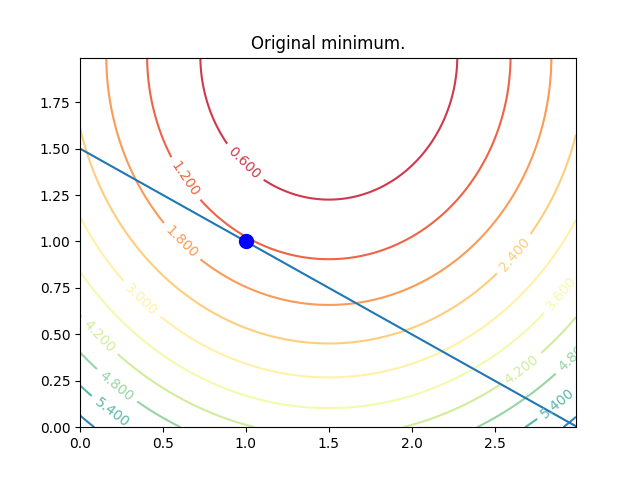
\includegraphics[width=.6\textwidth]{../img/original-minimum.png}
  \caption[Original minimum.]{Original minimum. \todo{remake figure}}\label{fig:original_minimum}
\end{figure}

Once one the agents attacks the system using~\eqref{eq:linear_attack_reprise}, the level curves are distorded, as seen in Fig.~\ref{fig:minimum_after_attack}.
This distortion changes the projection, resulting in a new constrained solution (in \todo{green}).
\begin{figure}[h]
  \centering
  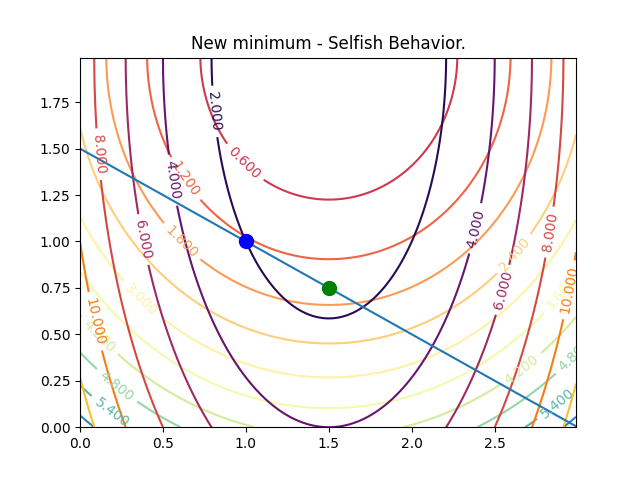
\includegraphics[width=.6\textwidth]{../img/new-minimum-selfish.png}
  \caption[Minimum after attack.]{Minimum after attack. \todo{remake figure}}\label{fig:minimum_after_attack}
\end{figure}

If the attacker is detected, one of our options to mitigate this drift is to substitute the $\lambdaicheat$ received during a negotiation by $\0$.
It can be interpreted as the coordinator punishing the attacker by assuming it will always be satisfied independent of the allocation given.
The negligence against the attacker will result in it receiving less and less resources. Asymptotically, the system will behave as the attacker was unplugged, since the negotiation will be maintained with the other agents, somehow similar to the examples in~\cite{VelardeEtAl2018,MaestreEtAl2021}.

In Fig.~\ref{fig:minimum_ignoring_attacker}, we see the new level curves and the new solution found (in \todo{magenta}) when ignoring the attacker.
\begin{figure}[h]
  \centering
  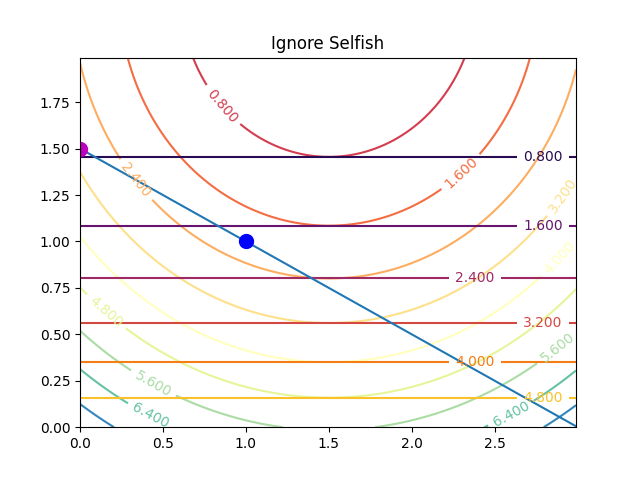
\includegraphics[width=.6\textwidth]{../img/ignoreX.png}
  \caption{Optimal value after ignoring attacker. \todo{remake figure}}\label{fig:minimum_ignoring_attacker}
\end{figure}

Although the idea of punishing the attacker by ignoring it may appear reasonably, since the system is a \cps{}, it may control some amenity that needs a minimal \QoS{}.
If we are controlling a \HVAC{} system, for instance, depending on the region of the planet, turning the heat off of the attacker could make the users extremely cold\todo{, as in the introductory example in Chapter~\ref{sec:introduction}}.

A solution would be to, before the negotiation, allocate minimal resources for the attacker, and then ignore it throughout the negotiation using the remainder of the resources, subtracting the maximum by the allocated for the attacker.
However, it would be needed to assess somehow what would be the fair amount to give to the attacker, which would not prejudice other agents.

We propose yet another solution, in which we try to recover the nominal behavior if some assumptions are guaranteed.
Passing from the level curves of the attacked system (Fig.~\ref{fig:minimum_after_attack}) to the shown in Fig.~\ref{fig:minimum_recovered}, where the new minimum lies in a neighboorhood of the original one (in Fig.~\ref{fig:original_minimum}).

\begin{figure}[h]
  \centering
  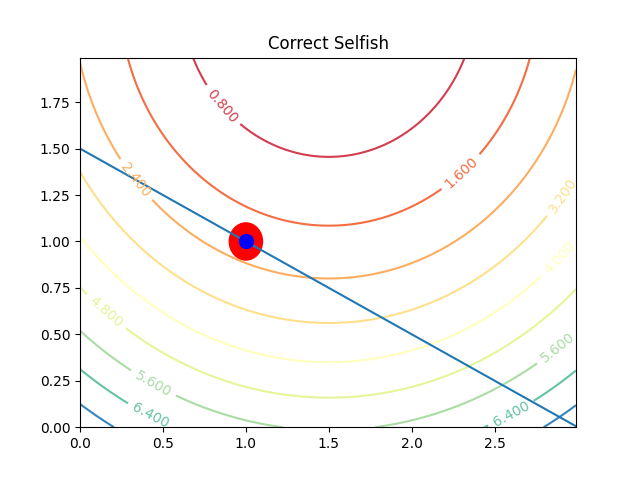
\includegraphics[width=.6\textwidth]{../img/correctX.png}
  \caption{Optimal value after trying to recover original behavior.}\label{fig:minimum_recovered}
\end{figure}

\subsubsection{Recovering nominal behavior}\label{sec:recov-nomin-behav}
If we observe the formula of the linear attack~\eqref{eq:linear_attack_reprise}, we can make some assumptions.

As seen in \S\ref{sec:example-interpr}, $\lambdai$ correspond to dissatisfaction with the allocation $\thetai$ given.
If $\lambdai=\0$, it means the agent is satisfied with the allocation.
So, we do not expect that the attacker will use a cheating matrix $\Tik$ that generates a $\lambdaicheat=\0$ when $\lambdai\neq\0$.

Given that we assume
\begin{equation}
  \left[\lambdaicheat=\0 \right] \implies \left[\lambdai=\0 \right],
\end{equation}
which translates to
\begin{equation}
  \lambdaicheat=\Tik\lambdai=\0\text{, only if }\lambdai=\0,
\end{equation}
which implies $\Tik$ is \textbf{invertible}.

Observing~\eqref{eq:lambda_function_theta_tilde}, we also assume that the choice of $\Tik$ does not change the structure of $\Plin$, i.e., $\Plintilde$ is also symmetric and thus also is $\Tik$.

Having the estimate $\Plintildeestimate$ and the nominal $\Plinnominal$ and using these assumptions, we can try to estimate the inverse of $\Tik$ using
\begin{equation}
{\Tikinvestimate=\Plinnominal{\Plintildeestimate}^{-1}}.
\end{equation}

And with the estimate $\Tikinvestimate$, we can try to reconstruct $\lambdai$:
\begin{equation}
  \label{eq:lambdareconstruction}
  \lambdaireconstructed=-\Plinnominal\thetai-\Tikinvestimate\siktildeestimate
\end{equation}

So, we can modulate the negotiation algorithm, by using $\lambdaimodified$ choosing what version of $\lambdai$ to choose, i.e.,
\begin{equation}
  \lambdaimodified=
          \begin{cases}
            \lambdaicheat, &\text{if } d_{i}=0\\
            \lambdaireconstructed, &\text{if }d_{i}=1\\
        \end{cases}
\end{equation}

\begin{remark}
  Observe that if estimate of $\Plin$ do not converge, we cannot reconstruct $\lambdaik$ so we need to use one of the other options proposed, ignore the attacker, or use minimal allocation.
  Since it may be difficult to asses the minimal allocation, we ignore the cases when the estimation does not converge.\note{or I can just ignore}
\end{remark}

\section{Complete safe dMPC for scarce systems}\label{sec:complete-safe-dmpc}
Compiling the detection and mitigation schemes described in the last sections, we can finally have our \rpdmpcss{}.
Algorithm~\ref{alg:rpdbdmpcss} systematizes the method.

% \begin{algorithm2e}[h]
%   \DontPrintSemicolon%
%   \coordinit{
%     Initialize $k$, $p$, $a$, $b$, $p_{\max}$ and $\epsilon$\;
%   }
%   \While{$k\geq 0$}{
%     Initialize ${\thetaik}^{(p)},$ $\forall i\in\set{M}$, such that ${\vec{\theta}[k]}^{(p)}\in\set{S}$\;
%     Coordinator sends $\thetaik^{(p)}$ for all agents\;
%     \exchange{
%       \Repeat{$\left[\norm{{\vec{\theta}[k]}^{(p)}-{\vec{\theta}[k]}^{(p-1)}}\leq\epsilon\right]\lor \left[p\geq p_{\max}\right]$}{
%         Agents solve local sub-problems~\eqref{eq:DOP_local} and send ${\vec{\lambda}_{i}[k]}^{(p)}$ to coordinator\;
%         Coordinator updates $\vec{\theta}[k]$ using~\eqref{eq:projectedSubgradient_lambda} and sends to local agents\;
%         $p\gets p+1$\;
%       }
%     }
%     Agents apply on respective sub-systems the last calculated $\vec{u}_{i}^{\star}[0|k]$\;
%     $k\gets k+1$\;
%   }
%   \caption{Primal decomposition-based \dmpc{}.}\label{alg:primal_decomposition_based_dmpc}
% \end{algorithm2e}
\begin{algorithm2e}[h]
  \DontPrintSemicolon
  \detectPhase{
  $h:=0$\;
    \Repeat{
$\|\eta_{i}^{h}-\eta^{h-1}\|\leq\epsilon$
}{
    Coordinator sets random $\vec{\theta}_{i}^{(h+1)}$ \;
    Subsystems solve~\eqref{eq:DOP_local}, and send $\vec{\lambda}^{\star}_{i}(\vec{\theta}^{(h)})$\;
    Coordinator estimates $\widehat{\tilde{P}}_{i}(k)^{(h)}$ and $\widehat{\tilde{\vec{s}}}_{i}(k)^{(h)}$ \;
    $h:=h+1$\;
    }
    Coordinator computes $d_{i}$ using~\eqref{eq:2}\;
  }
  \negotPhase{
  Coordinator initializes $\vec{\theta}^{(0)}$ \;
  $p:=0$\;

  \Repeat{$\|\vec{\theta}^{(p)} -\vec{\theta}^{(p-1)}\|\leq\epsilon$}{
  Subsystems solve~\eqref{eq:DOP_local}, and send $\vec{\lambda}^{\star}_{i}(\vec{\theta}\p)$\;

  Coordinator updates allocation~\eqref{eq:thetaNegot} using adequate versions of $\vec{\lambda}_{i}$ for each agent: $\vec{\lambda}_{i}^{\star}(\vec{\theta}\p)$, if $d_{i}=0$ and ${\vec{\lambda}_{i}}_{\mathrm{rec}}$, if ${d_{i}=1}$\;
  $p:=p+1$
 }}
 \caption{Resilient Primal Decomposition-based dMPC for scarce systems. \todo{rework algo}}\label{alg:rpdbdmpcss}
\end{algorithm2e}


\section{Numerical experiment}\label{sec:numerical-experiment}

We illustrate the operation of the resilient algorithm just presented with an academic example.
This example is more complex and based on reality than the others presented so far.
The case studied will be used for the rest of this work with some minor adjustments when needed (inclusion or suppression of assumptions).

\subsection{\dhnlong}\label{sec:case-study}
We analyze the case of a simple \dhn{} composed of ${M=4}$ distinct \todo{small sized} houses (called I, II, II and IV).
Each house has state $\vec{x}_{i}$, and a different temperature reference $\vec{w}_{i}(t)$ for the inside air (users have different needs).
The houses are equipped with convectors, and the total heating power consumed by each house is $\vec{u}_{i}(t)\succeq\0$.
In Fig.~\ref{fig:houses} we see the houses consuming from a centralized heat provider.

\begin{figure}[h]
  \centering
  \begin{tikzpicture}[node distance=1cm and 1cm,scale=1]
    \node[color=mpc_agent] (house1) at (0,0) {\scalebox{2.5}{\faHome}};
    \node[minimum height=1cm,below=of house1] (medium) {};
    \node[color=mpc_agent,right=of medium] (house2)  {\scalebox{3.5}{\faHome}};
    \node[color=mpc_agent,below=of medium] (house3)  {\scalebox{3}{\faHome}};
    \node[color=mpc_agent,left=5cm of medium] (house4)  {\scalebox{7}{\faHome}};

    \draw[latex-,line width=1pt] (house1) -- (medium.center);
    \draw[latex-,line width=1pt] (house2) -- (medium.center);
    \draw[latex-,line width=1pt] (house3) -- (medium.center);
    \draw[latex-,line width=1pt] (house4) -- (medium.center) node[above,midway] {\large $\vec{u}_{i}(t)$};
    \draw[color=black,fill=mpc_coordinator,] (medium) circle [radius=.2cm];

    \node[latex-,line width=7pt] at ($(house4) +(-1,1)$) {\large $w_{i}(t)$};
    \node[latex-,line width=7pt] at ($(house4)$) {$\vec{x}_{i}(t)$};

  \end{tikzpicture}
  \caption{District with 4 houses.}\label{fig:houses}
\end{figure}

To model each house, we can use the 3R-2C monozone model with a window~\cite{GoudaEtAl2002}, where the thermic elements are represented as equivalent electric elements in a 3 resistors, and 2 capacitors electric circuit.
The electric circuit is depicted in Fig.~\ref{fig:3R2C_model}.
Current sources are added to correspond to solar irradiation and the heating power.
A voltage source represents the temperature outside the house.
The meaning of each component is given in Tab.~\ref{tab:modelParamMeaning}, and the respective values for each one of the houses is given in Tab.~\ref{tab:modelParam}.

\begin{figure}[h]
  \centering
  \begin{circuitikz}[european]
    \draw (0,0) node[tlground]{} to[isource, l=$P^{\text{heat}}$] ++(0,2) to[short, -*] ++(1.5,0) coordinate (a);

    \draw (a) node[above]{$T^{\text{in}}$}  to[C=$C^{\text{air}}$] ++(0,-2) node[tlground]{};
    \draw (0,-3) node[tlground]{} to[isource, l=$I^{\text{sol}}$] ++(0,2)
    to[short, -*] ++(1.5,0) coordinate (b);
    \draw (b) to[C=$C^{\text{walls}}$] ++(0,-2) node[tlground]{};

    \draw (a) -- ++(2,0) coordinate (c) -- ++(0,-.5) to[R=$R^{\text{iw/ia}}$] ++(0,-2) -- ++(0,-.5) coordinate (d);

    \draw (b) node[above]{$T^{\text{walls}}$} to[short,-*] (d);

    \draw (c) --  ++(2.5,0) -- ++(0,-.5) to[R=$R^{\text{oa/ia}}$] ++(0,-2) -- ++(0,-.5) coordinate (e);

    \draw (d) to[R=$R^{\text{ow/oa}}$] (e) to[battery,l=$T^{\text{out}}$] ++(0,-2) node[tlground]{};
  \end{circuitikz}
  \caption{Thermic Model 3R-2C of a house. \todo{verify model}}\label{fig:3R2C_model}
\end{figure}

\begin{table}[h]
  \centering
  \caption{Model Parameters}\label{tab:modelParamMeaning}
  \begin{tabular}[b]{cl}
    \toprule
    Symbol&Meaning\\
    \midrule
    $C^{\text{air}}_{i}$  &Heat capacity of inside air\\
    $C^{\text{walls}}_{i}$ &Heat capacity of external walls\\
    $R^{\text{iw/ia}}_{i}$ &Resist.\ between inside air and inside walls\\
    $R^{\text{ow/oa}}_{i}$ &Resist.\ between outside air and outside walls\\
    $R^{\text{oa/ia}}_{i}$ &Resist.\ between inside and out.\ air (from windows)\\
    $P^{\text{heat}}$ &Convector's heating power\\
    $I^{\text{sol}}$ &Sun's heating Power (by irradiance)\\
    $T^{\text{in}}$ &Mean temperature of Inside Air\\
    $T^{\text{walls}}$ &Mean temperature of Inside Walls\\
    \bottomrule
  \end{tabular}
\end{table}

\begin{table}[h]
  \centering
  \caption{
    Parameters for each agent}\label{tab:modelParam}
  \begin{tabular}[t]{cccccc} \toprule
    Symbol& I & II & III & IV &Unit\\
    \midrule
    $C^{\text{walls}}$   &$5.4$&$4.9$&$4.7$&$4.7$ &$10^{4}\mathrm{J/K}$ \\
    $C^{\text{air}}$     &$7.5$ &$8.4 $&$8.2$ &$7.7$&$10^{4}\mathrm{J/K}$  \\
    $R^{\text{oa/ia}}$   &$5.2$&$4.6$&$4.9$&$5.4$&$10^{-3}\mathrm{K/W}$ \\
    $R^{\text{iw/ia}}$   &$2.3$&$2.4$&$2.3$&$2.9$&$10^{-4}\mathrm{K/W}$\\
    $R^{\text{ow/oa}}$   &$1.5$&$0.6$&$0.7$&$0.7$& $10^{-4}\mathrm{K/W}$ \\
    \bottomrule
  \end{tabular}
\end{table}


The electric circuit corresponds to a \ltict{} system, which can be represented in the state-space model by
\todo[verify]{
  \begin{equation}
  \begin{matrix}
    \label{eq:systems_cont}
    \dot{\vec{x}}_{i}(t)  &=&{A_{c}}_{i}\vec{x}_{i}(t) &+& {B_{c}}_{i}\vec{u}_{i}(t)+{D_{c}}_{i}\vec{d}_{i}(t)\\
    \vec{y}_{i}(t)        &=&{C_{c}}_{i}\vec{x}_{i}(t) &&
  \end{matrix},
\end{equation}
}
where
\todo[verify]{
\begin{equation}
  \label{eq:4}
  \begin{matrix}
    A_{\mathrm{c}_{i}}=\left[
    \begin{matrix}
      -\frac{1}{C^{\text{walls}}_{i}R^{\text{oa/ia}}_{i}}-\frac{1}{C^{\text{walls}}_{i}R^{\text{iw/ia}}_{i}}& \frac{1}{C^{\text{walls}}_{i}R^{\text{iw/ia}}_{i}}\\
      \frac{1}{C^{\text{air}}_{i}R^{\text{iw/ia}}_{i}} &-\frac{1}{C^{\text{air}}_{i}R^{\text{ow/oa}}o_{i}}-\frac{1}{C^{\text{air}}_{i}R^{\text{iw/ia}}_{i}}
    \end{matrix}\right]
                                                         &
      B_{\mathrm{c}_{i}}=\left[\begin{matrix}  \frac{P^{\text{heat}}}{C^{\text{air}}_{i}}\\ 0\end{matrix}\right]\T
  \\\\
    D_{\mathrm{c}_{i}}=\left[
    \begin{matrix}
      0& \frac{1}{C^{\text{air}}_{i}R^{\text{ow/oa}}_{i}}\\
      \frac{1}{C^{\text{air}}_{i}} &\frac{1}{C^{\text{air}}_{i}R^{\text{ow/oa}}}
    \end{matrix}\right]&C_{\mathrm{c}_{i}}=\left[\begin{matrix}1 & 0\end{matrix}\right]

\end{matrix}
\end{equation}
}
where
${\vec{x}_{i}(t)=\left[T^{\text{in}}_{i}(t)\ T^{\text{walls}}_{i}(t)\right]\T}$,
${\vec{u}_{i}(t)=P^{\text{heat}}_{i}}$,
${\vec{d}_{i}(t)=\left[I^{\text{sol}}(t)\ T^{\text{out}}(t)\right]\T}$.

Their heating inputs $\vec{u}_{i}(t)$ are constraint by the maximum heat power such
\begin{equation}
\sum\limits_{i\in\set{M}}\left[\vec{u}_{i}(t)\right]\preceq \vec{u}_{\max}
\end{equation}
with
\todo{$\vec{u}_{\max}=4\mathrm{kW}$}
.

\begin{remark}
  For our examples, we ignore the disturbances caused by the outside temperature and the sun, i.e., $\vec{d}_{i}(t)=\0$.
\end{remark}

We want to control the system using \mpc{}, so we discretize the system using a zero-order holder and sampling time of $T_{s}=0.25\mathrm{h}$, resulting in the $3$-tuples $(A_{i},B_{i},C_{i})$.

\subsection{Applying \rpdmpcss{}}
First, to use the \rpdmpcss{}, we assume the houses have references $\vec{w}_{i}[k]$ which cannot be achieved given an initial state $\vec{x}_{i}[0]$, due to input constraints.

For example, we suppose they have initial states
\todo[use from simulation]{
  $\vec{x}_{\text{I}}[0]=$,
  $\vec{x}_{\text{II}}[0]=$,
  $\vec{x}_{\text{III}}[0]=$,
  and
  $\vec{x}_{\text{IV}}[0]=$
}
, and references
\todo[use from simulation]{
  $w_{\text{I}}[0]=$,
  $w_{\text{II}}[0]=$,
  $w_{\text{III}}[0]=$,
  and
  $w_{\text{IV}}[0]=$
}.
Using gains
$Q=10I$


\subsubsection{Results}\label{sec:results}

\begin{figure}[h]
  \centering
  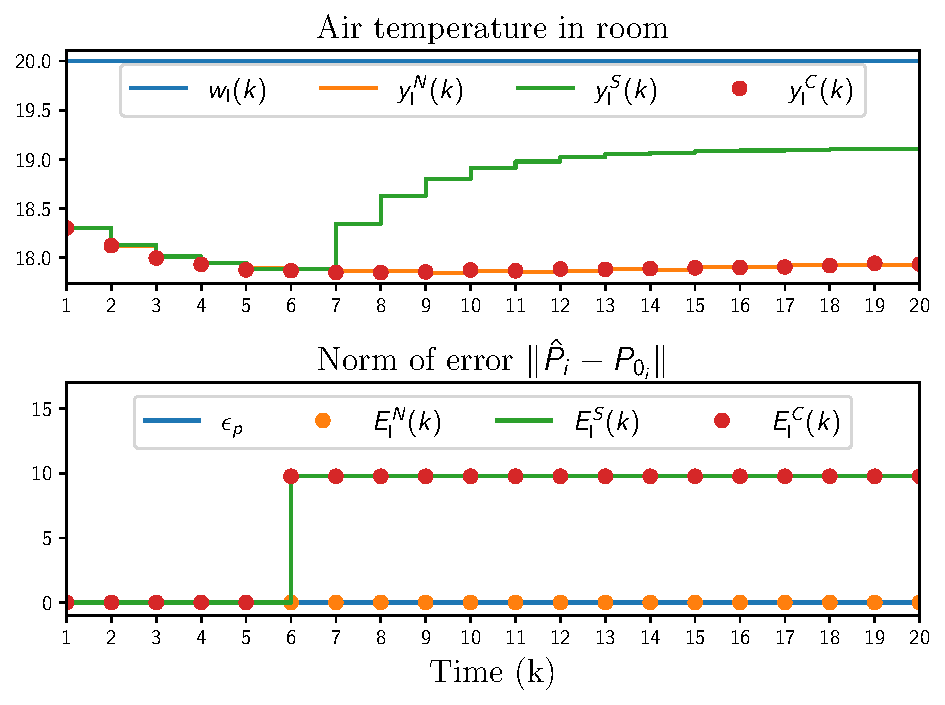
\includegraphics[width=7cm]{AirTempAndDecisionVariable.pdf}
\caption{Air temperature in room I and the decision variable $E_{I}(k)$ for
different scenarios: nominal (N), with selflish behavior without correction (S)
and with selfish behavior with correction (C)}\label{fig:response3Scenarios}
\end{figure}

\begin{table}[t]
  \centering
  \caption{Comparison of costs $J_{i}^{N}$ and $J_{G}^{N}$}\label{tab:costsGlobalLocal}
  \begin{tabular}[t]{cccc} \toprule
    Agent  & Nominal & Selfish & Selfish + correction\\
    \midrule
    I      & 103  &  64  & 104  \\
    II     &  73  &  91  &  73  \\
    III    & 100  & 123  & 101  \\
    IV     & 132  & 154  & 131  \\
    Global & 408  & 442  & 409  \\
    \bottomrule
  \end{tabular}
\end{table}

\end{document}
